
Para el análisis consideramos necesario experimentar únicamente aumentando el valor de entrada, ya que no tenemos ni mejor ni peor caso porque el algoritmo recorre sin excepciones todo el vector una cantidad logarítmica de veces. 

Realizamos las mediciones para un rango de $N$ entre $1$ y $10000$. Se obtuvo el siguiente gráfico:

\begin{figure}[h]
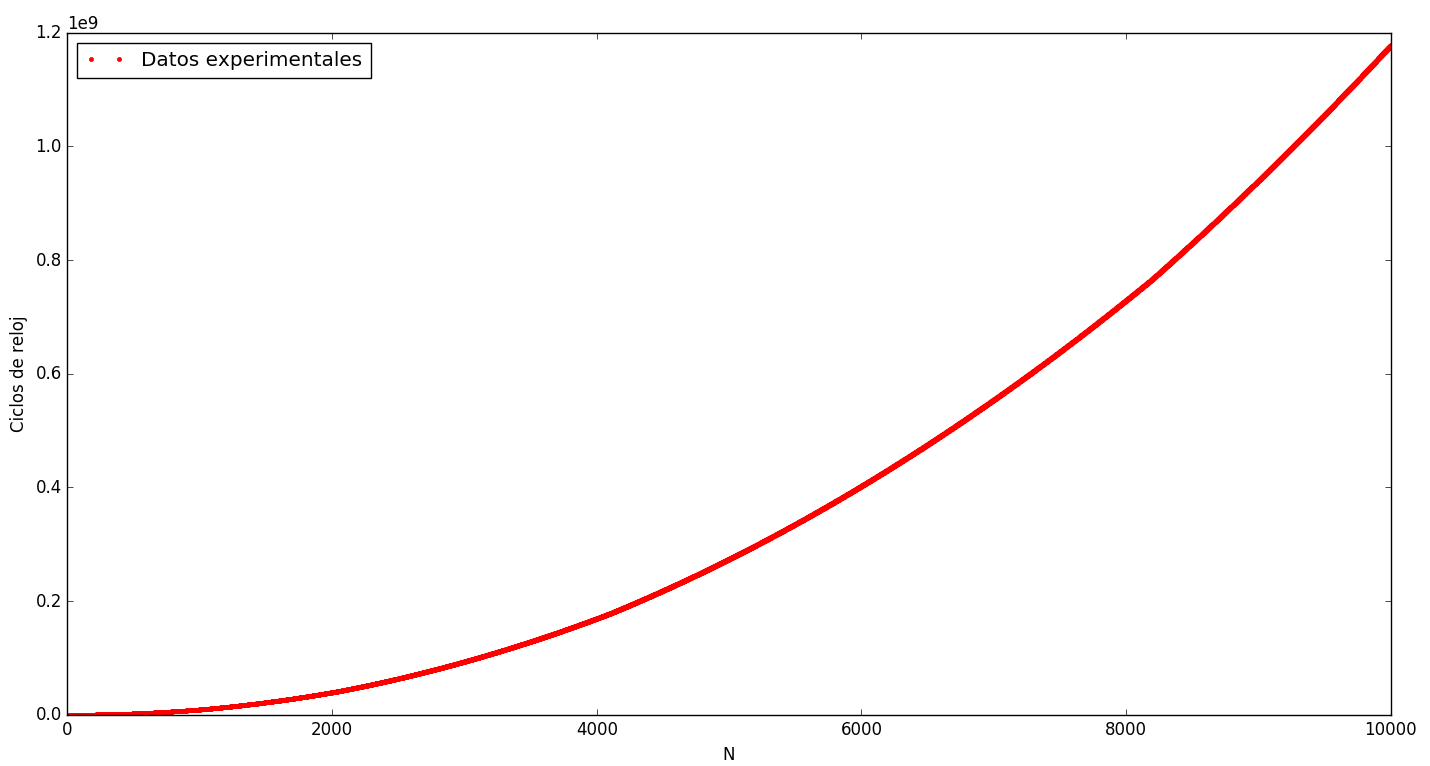
\includegraphics[width=\textwidth]{p1}
\caption{Gráfico obtenido a partir de las mediciones realizadas para el problema 1}
\end{figure}

Se observa que, como esperábamos, la cantidad de ciclos de reloj aumenta con $N$.
% TODO trata de frutear algo mas (aca es donde no dio el ajuste >n<)